\section{Exercise C.}
Consider this diagram:\\

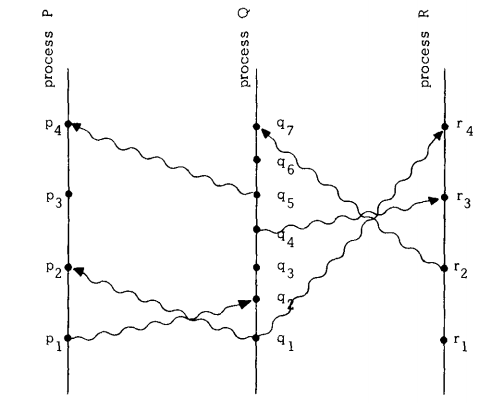
\includegraphics[scale=0.7]{ExerciseC-processDiagram}\\
\begin{enumerate}
\item Write out the happens-before relation in the following diagram. (Immediate successors is fine; you don’t have to write the entire transitive closure.
\item Identify 4 consistent cuts.
\item Identify 4 inconsistent cuts.
\item Write 2 different linearizations of the events in this diagram.
\end{enumerate}

\textbf{1) Happens before successors.}\\
\begin{tabular}{ l r }
\hline \\[0.1cm]
q1->q2->q3->q4->q5->q6->q7 	& HB statement 1 \\[0.1cm]
p1->p2->p3->p4 				& HB statement 1 \\[0.1cm]
r1->r2->r3->r4 				& HB statement 1 \\[0.1cm]
\hline \\[0.1cm]
p1->q2 & HB statement 2 \\[0.1cm]
q1->p2 & HB statement 2 \\[0.1cm]
q1->r4 & HB statement 2 \\[0.1cm]
q4->r3 & HB statement 2 \\[0.1cm]
q5->p4 & HB statement 2 \\[0.1cm]
r2->q7 & HB statement 2 \\[0.1cm]
\hline 
\end{tabular}\\\\

\textbf{2) Consistent cuts}\\
\begin{tabular}{ l l l }
Process P & Procces Q & Process R \\[0.1cm]
\hline 
p1 		& q1 	& r1 	\\[0.1cm]
p1-p3 	& q1-q4 & r1-r4 \\[0.1cm]
p1 		& q1-q7 & r1-r2 \\[0.1cm]
p1-p4 	& q1-q7 & r1-r4 \\[0.1cm]
\hline 
\end{tabular}\\\\

\textbf{2) Inconsistent cuts}\\
\begin{tabular}{ l l l | l }
Process P & Procces Q & Process R & Explanation \\[0.1cm]
\hline 
p1-p4 	& q1 	& r1 	& q5->p4 			\\[0.1cm]
p1-p3 	& q1-q2 & r1-r4 & q4->r3 , vr3-> r4 \\[0.1cm]
p1 		& q1-q7 & r1 	& r2->q7 			\\[0.1cm]
p1-2	& none 	& r1-r4 & q1->p2, q1->r4 	\\[0.1cm]
\hline 
\end{tabular}\\\\

\newpage